\documentclass[11pt,addpoints,answers]{exam}

%-----------------------------------------------------------------------------
% PACKAGES AND OTHER DOCUMENT CONFIGURATIONS
%-----------------------------------------------------------------------------

\usepackage[margin=1in]{geometry}
\usepackage{amsmath, amsfonts}
\usepackage{enumerate}
\usepackage{graphicx}
\usepackage{titling}
\usepackage{url}
\usepackage{xfrac}
\usepackage{natbib}
\usepackage{amssymb}
\usepackage{amsthm}
\usepackage{paralist}
\usepackage{epstopdf}
\usepackage{tabularx}
\usepackage{longtable}
\usepackage{multirow}
\usepackage{multicol}
\usepackage[colorlinks=true,urlcolor=blue]{hyperref}
\usepackage{algorithm}
\usepackage{algorithmicx}
\usepackage[noend]{algpseudocode}
\usepackage{float}
\usepackage{enumerate}
\usepackage{array}
\usepackage{environ}
\usepackage{times}
\usepackage{textcomp}
\usepackage{caption}
\usepackage{parskip} % For NIPS style paragraphs.
\usepackage[compact]{titlesec} % Less whitespace around titles
\usepackage[inline]{enumitem} % For inline enumerate* and itemize*
\usepackage{datetime}
\usepackage{comment}
% \usepackage{minted}
\usepackage{lastpage}
\usepackage{color}
\usepackage{xcolor}
\usepackage[final]{listings}
\usepackage{tikz}
\usetikzlibrary{shapes,decorations}
\usepackage{framed}
\usepackage{booktabs}
\usepackage{cprotect}
\usepackage{verbatim}
\usepackage{verbatimbox}
\usepackage{multicol}
\usepackage{hyperref}
\usepackage{subcaption}
\usepackage{mathtools} % For drcases
\usepackage{cancel}
\usepackage[many]{tcolorbox}
\usepackage{soul}
\usepackage[bottom]{footmisc}
\usepackage{bm}
\usepackage{wasysym}
\usepackage[utf8]{inputenc}
\usepackage{tikz}
\usetikzlibrary{arrows}
\usetikzlibrary{arrows.meta}
\usetikzlibrary{shapes.geometric}
\usetikzlibrary{positioning, arrows, automata, calc}
\usepackage{transparent}

\newtcolorbox[]{your_solution}[1][]{
    % breakable,
    enhanced,
    nobeforeafter,
    colback=white,
    title=Your Answer,
    sidebyside align=top,
    box align=top,
    #1
}

%%%%%%%%%%%%%%%%%%%%%%%%%%%%%%%%%%%%%%%%%%%
% Formatting for \CorrectChoice of "exam" %
%%%%%%%%%%%%%%%%%%%%%%%%%%%%%%%%%%%%%%%%%%%

\CorrectChoiceEmphasis{}
\checkedchar{\blackcircle}

%%%%%%%%%%%%%%%%%%%%%%%%%%%%%%%%%%%%%%%%%%%
% Rotated Column Headers                  %
%%%%%%%%%%%%%%%%%%%%%%%%%%%%%%%%%%%%%%%%%%%
\usepackage{adjustbox}
\usepackage{array}

%https://tex.stackexchange.com/questions/32683/rotated-column-titles-in-tabular

\newcolumntype{R}[2]{%
    >{\adjustbox{angle=#1,lap=\width-(#2)}\bgroup}%
    l%
    <{\egroup}%
}
\newcommand*\rot{\multicolumn{1}{R{45}{1em}}}% no optional argument here, please!

%%%%%%%%%%%%%%%%%%%%%%%%%%%%%%%%%%%%%%%%%%
% Custom commands                        %
%%%%%%%%%%%%%%%%%%%%%%%%%%%%%%%%%%%%%%%%%%

\newcommand{\vc}[1]{\boldsymbol{#1}}
\newcommand{\adj}[1]{\frac{d J}{d #1}}
\newcommand{\chain}[2]{\adj{#2} = \adj{#1}\frac{d #1}{d #2}}

\newcommand{\R}{\mathbb{R}}
\newcommand{\blackcircle}{\tikz\draw[black,fill=black] (0,0) circle (1ex);}
\renewcommand{\circle}{\tikz\draw[black] (0,0) circle (1ex);}

\newcommand{\emptysquare}{{\LARGE $\square$}\ \ }
\newcommand{\filledsquare}{{\LARGE $\blacksquare$}\ \ }
\newcommand{\emptycircle}{{\LARGE $\fullmoon$}\ \ }
\newcommand{\filledcircle}{{\LARGE $\newmoon$}\ \ }

\newcommand{\ntset}{test}

% mathcal
\newcommand{\Ac}{\mathcal{A}}
\newcommand{\Bc}{\mathcal{B}}
\newcommand{\Cc}{\mathcal{C}}
\newcommand{\Dc}{\mathcal{D}}
\newcommand{\Ec}{\mathcal{E}}
\newcommand{\Fc}{\mathcal{F}}
\newcommand{\Gc}{\mathcal{G}}
\newcommand{\Hc}{\mathcal{H}}
\newcommand{\Ic}{\mathcal{I}}
\newcommand{\Jc}{\mathcal{J}}
\newcommand{\Kc}{\mathcal{K}}
\newcommand{\Lc}{\mathcal{L}}
\newcommand{\Mc}{\mathcal{M}}
\newcommand{\Nc}{\mathcal{N}}
\newcommand{\Oc}{\mathcal{O}}
\newcommand{\Pc}{\mathcal{P}}
\newcommand{\Qc}{\mathcal{Q}}
\newcommand{\Rc}{\mathcal{R}}
\newcommand{\Sc}{\mathcal{S}}
\newcommand{\Tc}{\mathcal{T}}
\newcommand{\Uc}{\mathcal{U}}
\newcommand{\Vc}{\mathcal{V}}
\newcommand{\Wc}{\mathcal{W}}
\newcommand{\Xc}{\mathcal{X}}
\newcommand{\Yc}{\mathcal{Y}}
\newcommand{\Zc}{\mathcal{Z}}

% mathbb
\newcommand{\Ab}{\mathbb{A}}
\newcommand{\Bb}{\mathbb{B}}
\newcommand{\Cb}{\mathbb{C}}
\newcommand{\Db}{\mathbb{D}}
\newcommand{\Eb}{\mathbb{E}}
\newcommand{\Fb}{\mathbb{F}}
\newcommand{\Gb}{\mathbb{G}}
\newcommand{\Hb}{\mathbb{H}}
\newcommand{\Ib}{\mathbb{I}}
\newcommand{\Jb}{\mathbb{J}}
\newcommand{\Kb}{\mathbb{K}}
\newcommand{\Lb}{\mathbb{L}}
\newcommand{\Mb}{\mathbb{M}}
\newcommand{\Nb}{\mathbb{N}}
\newcommand{\Ob}{\mathbb{O}}
\newcommand{\Pb}{\mathbb{P}}
\newcommand{\Qb}{\mathbb{Q}}
\newcommand{\Rb}{\mathbb{R}}
\newcommand{\Sb}{\mathbb{S}}
\newcommand{\Tb}{\mathbb{T}}
\newcommand{\Ub}{\mathbb{U}}
\newcommand{\Vb}{\mathbb{V}}
\newcommand{\Wb}{\mathbb{W}}
\newcommand{\Xb}{\mathbb{X}}
\newcommand{\Yb}{\mathbb{Y}}
\newcommand{\Zb}{\mathbb{Z}}

% mathbf lowercase
\newcommand{\av}{\mathbf{a}}
\newcommand{\bv}{\mathbf{b}}
\newcommand{\cv}{\mathbf{c}}
\newcommand{\dv}{\mathbf{d}}
\newcommand{\ev}{\mathbf{e}}
\newcommand{\fv}{\mathbf{f}}
\newcommand{\gv}{\mathbf{g}}
\newcommand{\hv}{\mathbf{h}}
\newcommand{\iv}{\mathbf{i}}
\newcommand{\jv}{\mathbf{j}}
\newcommand{\kv}{\mathbf{k}}
\newcommand{\lv}{\mathbf{l}}
\newcommand{\mv}{\mathbf{m}}
\newcommand{\nv}{\mathbf{n}}
\newcommand{\ov}{\mathbf{o}}
\newcommand{\pv}{\mathbf{p}}
\newcommand{\qv}{\mathbf{q}}
\newcommand{\rv}{\mathbf{r}}
\newcommand{\sv}{\mathbf{s}}
\newcommand{\tv}{\mathbf{t}}
\newcommand{\uv}{\mathbf{u}}
\newcommand{\vv}{\mathbf{v}}
\newcommand{\wv}{\mathbf{w}}
\newcommand{\xv}{\mathbf{x}}
\newcommand{\yv}{\mathbf{y}}
\newcommand{\zv}{\mathbf{z}}

% mathbf uppercase
\newcommand{\Av}{\mathbf{A}}
\newcommand{\Bv}{\mathbf{B}}
\newcommand{\Cv}{\mathbf{C}}
\newcommand{\Dv}{\mathbf{D}}
\newcommand{\Ev}{\mathbf{E}}
\newcommand{\Fv}{\mathbf{F}}
\newcommand{\Gv}{\mathbf{G}}
\newcommand{\Hv}{\mathbf{H}}
\newcommand{\Iv}{\mathbf{I}}
\newcommand{\Jv}{\mathbf{J}}
\newcommand{\Kv}{\mathbf{K}}
\newcommand{\Lv}{\mathbf{L}}
\newcommand{\Mv}{\mathbf{M}}
\newcommand{\Nv}{\mathbf{N}}
\newcommand{\Ov}{\mathbf{O}}
\newcommand{\Pv}{\mathbf{P}}
\newcommand{\Qv}{\mathbf{Q}}
\newcommand{\Rv}{\mathbf{R}}
\newcommand{\Sv}{\mathbf{S}}
\newcommand{\Tv}{\mathbf{T}}
\newcommand{\Uv}{\mathbf{U}}
\newcommand{\Vv}{\mathbf{V}}
\newcommand{\Wv}{\mathbf{W}}
\newcommand{\Xv}{\mathbf{X}}
\newcommand{\Yv}{\mathbf{Y}}
\newcommand{\Zv}{\mathbf{Z}}

% bold greek lowercase
\newcommand{\alphav     }{\boldsymbol \alpha     }
\newcommand{\betav      }{\boldsymbol \beta      }
\newcommand{\gammav     }{\boldsymbol \gamma     }
\newcommand{\deltav     }{\boldsymbol \delta     }
\newcommand{\epsilonv   }{\boldsymbol \epsilon   }
\newcommand{\varepsilonv}{\boldsymbol \varepsilon}
\newcommand{\zetav      }{\boldsymbol \zeta      }
\newcommand{\etav       }{\boldsymbol \eta       }
\newcommand{\thetav     }{\boldsymbol \theta     }
\newcommand{\varthetav  }{\boldsymbol \vartheta  }
\newcommand{\iotav      }{\boldsymbol \iota      }
\newcommand{\kappav     }{\boldsymbol \kappa     }
\newcommand{\varkappav  }{\boldsymbol \varkappa  }
\newcommand{\lambdav    }{\boldsymbol \lambda    }
\newcommand{\muv        }{\boldsymbol \mu        }
\newcommand{\nuv        }{\boldsymbol \nu        }
\newcommand{\xiv        }{\boldsymbol \xi        }
\newcommand{\omicronv   }{\boldsymbol \omicron   }
\newcommand{\piv        }{\boldsymbol \pi        }
\newcommand{\varpiv     }{\boldsymbol \varpi     }
\newcommand{\rhov       }{\boldsymbol \rho       }
\newcommand{\varrhov    }{\boldsymbol \varrho    }
\newcommand{\sigmav     }{\boldsymbol \sigma     }
\newcommand{\varsigmav  }{\boldsymbol \varsigma  }
\newcommand{\tauv       }{\boldsymbol \tau       }
\newcommand{\upsilonv   }{\boldsymbol \upsilon   }
\newcommand{\phiv       }{\boldsymbol \phi       }
\newcommand{\varphiv    }{\boldsymbol \varphi    }
\newcommand{\chiv       }{\boldsymbol \chi       }
\newcommand{\psiv       }{\boldsymbol \psi       }
\newcommand{\omegav     }{\boldsymbol \omega     }

% bold greek uppercase
\newcommand{\Gammav     }{\boldsymbol \Gamma     }
\newcommand{\Deltav     }{\boldsymbol \Delta     }
\newcommand{\Thetav     }{\boldsymbol \Theta     }
\newcommand{\Lambdav    }{\boldsymbol \Lambda    }
\newcommand{\Xiv        }{\boldsymbol \Xi        }
\newcommand{\Piv        }{\boldsymbol \Pi        }
\newcommand{\Sigmav     }{\boldsymbol \Sigma     }
\newcommand{\Upsilonv   }{\boldsymbol \Upsilon   }
\newcommand{\Phiv       }{\boldsymbol \Phi       }
\newcommand{\Psiv       }{\boldsymbol \Psi       }
\newcommand{\Omegav     }{\boldsymbol \Omega     }

%%%%%%%%%%%%%%%%%%%%%%%%%%%%%%%%%%%%%%%%%%%
% Code highlighting with listings         %
%%%%%%%%%%%%%%%%%%%%%%%%%%%%%%%%%%%%%%%%%%%

\definecolor{bluekeywords}{rgb}{0.13,0.13,1}
\definecolor{greencomments}{rgb}{0,0.5,0}
\definecolor{redstrings}{rgb}{0.9,0,0}
\definecolor{light-gray}{gray}{0.95}

\newcommand{\MYhref}[3][blue]{\href{#2}{\color{#1}{#3}}}%

\definecolor{dkgreen}{rgb}{0,0.6,0}
\definecolor{gray}{rgb}{0.5,0.5,0.5}
\definecolor{mauve}{rgb}{0.58,0,0.82}

\lstdefinelanguage{Shell}{
  keywords={tar, cd, make},
  %keywordstyle=\color{bluekeywords}\bfseries,
  alsoletter={+},
  ndkeywords={python, py, javac, java, gcc, c, g++, cpp, .txt, octave, m, .tar},
  %ndkeywordstyle=\color{bluekeywords}\bfseries,
  identifierstyle=\color{black},
  sensitive=false,
  comment=[l]{//},
  morecomment=[s]{/*}{*/},
  commentstyle=\color{purple}\ttfamily,
  %stringstyle=\color{red}\ttfamily,
  morestring=[b]',
  morestring=[b]",
  backgroundcolor = \color{light-gray}
}

\lstset{columns=fixed, basicstyle=\ttfamily,
    backgroundcolor=\color{light-gray},xleftmargin=0.5cm,frame=tlbr,framesep=4pt,framerule=0pt}


%%%%%%%%%%%%%%%%%%%%%%%%%%%%%%%%%%%%%%%%%%%
% Custom box for highlights               %
%%%%%%%%%%%%%%%%%%%%%%%%%%%%%%%%%%%%%%%%%%%

% Define box and box title style
\tikzstyle{mybox} = [fill=blue!10, very thick,
    rectangle, rounded corners, inner sep=1em, inner ysep=1em]

% \newcommand{\notebox}[1]{
% \begin{tikzpicture}
% \node [mybox] (box){%
%     \begin{minipage}{\textwidth}
%     #1
%     \end{minipage}
% };
% \end{tikzpicture}%
% }

\NewEnviron{notebox}{

\begin{tikzpicture}
\node [mybox] (box){
    \begin{minipage}{\textwidth}
        \BODY
    \end{minipage}
};
\end{tikzpicture}
}

%%%%%%%%%%%%%%%%%%%%%%%%%%%%%%%%%%%%%%%%%%%
% Commands showing / hiding solutions     %
%%%%%%%%%%%%%%%%%%%%%%%%%%%%%%%%%%%%%%%%%%%

%% To HIDE SOLUTIONS (to post at the website for students), set this value to 0: 
\def\issoln{0}
% Some commands to allow solutions to be embedded in the assignment file.
\ifcsname issoln\endcsname \else \def\issoln{1} \fi
% Default to an empty solutions environ.
\NewEnviron{soln}{}{}
\if\issoln 1
% Otherwise, include solutions as below.
\RenewEnviron{soln}{
    \leavevmode\color{red}\ignorespaces
    % \textbf{Solution} \BODY
    \BODY
}{}
\fi

%% qauthor environment:
% Default to an empty qauthor environ.
\NewEnviron{qauthor}{}{}
%% To HIDE TAGS set this value to 0:
\def\showtags{0}
%%%%%%%%%%%%%%%%
\ifcsname showtags\endcsname \else \def\showtags{1} \fi
% Default to an empty tags environ.
\NewEnviron{tags}{}{}
\if\showtags 1
% Otherwise, include solutions as below.
\RenewEnviron{tags}{
    \fbox{
    \leavevmode\color{blue}\ignorespaces
    \textbf{TAGS:} \texttt{\url{\BODY}}
    }
    \vspace{-.5em}
}{}
\fi

%%%%%%%%%%%%%%%%%%%%%%%%%%%%%%%%%%%%%%%%%%%
% Commands for customizing the assignment %
%%%%%%%%%%%%%%%%%%%%%%%%%%%%%%%%%%%%%%%%%%%

\newcommand{\courseName}{10-301/10-601 Introduction to Machine Learning (Summer 2023)}
\newcommand{\hwName}{Programming Assignment 3: Logistic Regression}
\newcommand{\dueDate}{Thursday, June 15th}

\title{\textsc{\hwName}
%\thanks{Compiled on \today{} at \currenttime{}}
} % Title

\author{\courseName\\
\url{https://www.cs.cmu.edu/~hchai2/courses/10601/} \\
OUT: Thursday, June 8th \\
DUE: \dueDate{} \\ 
TAs: Alex, Andrew, Sofia, Tara, Markov, Neural the Narwhal
}

\newcommand{\homeworktype}{\string written/programming}

\date{}

%%%%%%%%%%%%%%%%%%%%%%%%%%%%%%%%%%%%%%%%%%%%%%%%%
% Useful commands for typesetting the questions %
%%%%%%%%%%%%%%%%%%%%%%%%%%%%%%%%%%%%%%%%%%%%%%%%%

\newcommand \expect {\mathbb{E}}
\newcommand \mle [1]{{\hat #1}^{\rm MLE}}
\newcommand \map [1]{{\hat #1}^{\rm MAP}}
\newcommand \argmax {\operatorname*{argmax}}
\newcommand \argmin {\operatorname*{argmin}}
\newcommand \code [1]{{\tt #1}}
\newcommand \datacount [1]{\#\{#1\}}
\newcommand \ind [1]{\mathbb{I}\{#1\}}

%%%%%%%%%%%%%%%%%%%%%%%%%%
% Document configuration %
%%%%%%%%%%%%%%%%%%%%%%%%%%

% Don't display a date in the title and remove the white space
\predate{}
\postdate{}
\date{}

% Don't display an author and remove the white space
%\preauthor{}
%\postauthor{}

% Solo and group questions
\newcommand{\solo}{\textbf{[SOLO]} }
\newcommand{\group}{\textbf{[GROUP]} }

% Question type commands
\newcommand{\sall}{\textbf{Select all that apply: }}
\newcommand{\sone}{\textbf{Select one: }}
\newcommand{\tf}{\textbf{True or False: }}

% AdaBoost commands
\newcommand{\trainerr}[1]{\hat{\epsilon}_S \left(#1\right)}
\newcommand{\generr}[1]{\epsilon \left(#1\right)}
\newcommand{\D}{\mathcal{D}}
\newcommand{\margin}{\text{margin}}
\newcommand{\sign}{\text{sign}}
\newcommand{\PrS}{\hat{\Pr_{(x_i, y_i) \sim S}}}
\newcommand{\PrSinline}{\hat{\Pr}_{(x_i, y_i) \sim S}}  % inline PrS

% Abhi messing around with examdoc
\qformat{\textbf{{\Large \thequestion \; \; \thequestiontitle \ (\totalpoints \ points)}} \hfill}
\renewcommand{\thequestion}{\arabic{question}}
\renewcommand{\questionlabel}{\thequestion.}

\renewcommand{\thepartno}{\arabic{partno}}
\renewcommand{\partlabel}{\thepartno.}
\renewcommand{\partshook}{\setlength{\leftmargin}{0pt}}

\renewcommand{\thesubpart}{\alph{subpart}}
\renewcommand{\subpartlabel}{(\thesubpart)}

\renewcommand{\thesubsubpart}{\roman{subsubpart}}
\renewcommand{\subsubpartlabel}{\thesubsubpart.}

% copied from stack overflow, as all good things are
\newcommand\invisiblesection[1]{%
  \refstepcounter{section}%
  \addcontentsline{toc}{section}{\protect\numberline{\thesection}#1}%
  \sectionmark{#1}}

% quite possibly the worst workaround i have made for this class
\newcommand{\sectionquestion}[1]{
\titledquestion{#1}
\invisiblesection{#1}
~\vspace{-1em}
}

%%%%%%%%%%%%%%%%%%%%%%%%%%%%%%%%%%%%%%%%%%%
% New Environment for Pseudocode          %
%%%%%%%%%%%%%%%%%%%%%%%%%%%%%%%%%%%%%%%%%%%

% Python style for highlighting
\DeclareFixedFont{\ttb}{T1}{txtt}{bx}{n}{12} % for bold
\DeclareFixedFont{\ttm}{T1}{txtt}{m}{n}{12}  % for normal

\definecolor{deepblue}{rgb}{0,0,0.5}
\definecolor{deepred}{rgb}{0.6,0,0}
\definecolor{deepgreen}{rgb}{0,0.5,0}

\newcommand\pythonstyle{\lstset{
language=Python,
basicstyle=\ttm,
morekeywords={self},              % Add keywords here
keywordstyle=\ttb\color{deepblue},
emph={MyClass,__init__},          % Custom highlighting
emphstyle=\ttb\color{deepred},    % Custom highlighting style
stringstyle=\color{deepgreen},
frame=tb,                         % Any extra options here
showstringspaces=false
}}


% Python environment
\lstnewenvironment{your_code_solution}[1][]
{
\pythonstyle
\lstset{#1}
}
{}


%%%%%%%%%%%%%%%%%%
% Begin Document %
%%%%%%%%%%%%%%%%%% 

\begin{document}

\maketitle

\begin{notebox}
\paragraph{Summary} In this assignment, you will build a sentiment polarity analyzer, which will be capable of analyzing the overall sentiment polarity (positive or negative) for restaurant reviews using logistic regression. In the written component, you will study linear and logistic regression.
\end{notebox}
\section*{START HERE: Instructions}
\begin{itemize}
\item \textbf{Collaboration policy:} Collaboration on solving the homework is allowed, after you have thought about the problems on your own. It is also OK to get clarification (but not solutions) from books or online resources, again after you have thought about the problems on your own. There are two requirements: first, cite your collaborators fully and completely (e.g., ``Jane explained to me what is asked in Question 2.1''). Second, write your solution {\em independently}: close the book and all of your notes, and send collaborators out of the room, so that the solution comes from you only.  See the Academic Integrity Section on the course site for more information: \url{https://www.cs.cmu.edu/~hchai2/courses/10601/}

\item\textbf{Late Submission Policy:} See the late submission policy here: \url{https://www.cs.cmu.edu/~hchai2/courses/10601/}

\item\textbf{Submitting your work:} 

\begin{itemize}

% Since we are not using Canvas this semester.
% \item \textbf{Canvas:} We will use an online system called Canvas for short answer and multiple choice questions. You can log in with your Andrew ID and password. (As a reminder, never enter your Andrew password into any website unless you have first checked that the URL starts with "https://" and the domain name ends in ".cmu.edu" -- but in this case it's OK since both conditions are met).  You may only \textbf{submit once} on canvas, so be sure of your answers before you submit.  However, canvas allows you to work on your answers and then close out of the page and it will save your progress.  You will not be granted additional submissions, so please be confident of your solutions when you are submitting your assignment.

\item \textbf{Programming:} You will submit your code for programming questions on the homework to Gradescope (\url{https://gradescope.com}). After uploading your code, our grading scripts will autograde your assignment by running your program on a virtual machine (VM). When you are developing, check that the version number of the programming language environment (e.g. Python 3.9.12) and versions of permitted libraries (e.g.  \texttt{numpy} 1.23.0) match those used on Gradescope. You have a \textbf{total of 10 Gradescope programming submissions.} Use them wisely. In order to not waste code submissions, we recommend debugging your implementation on your local machine (or the linux servers) and making sure your code is running correctly first before any Gradescope coding submission.

\item \textbf{Written:} For written problems such as short answer, multiple choice, derivations, proofs, or plots, please use the provided template. You must typeset your submission using \LaTeX{}. If your submission is misaligned with the template, there will be a \textbf{\textcolor{red}{2\% penalty}} (e.g., if the homework is out of 100 points, 2 points will be deducted from your final score). Each derivation/proof should be completed in the boxes provided. Do not move or resize any of the answer boxes. If you do not follow the template, your assignment may not be graded correctly by our AI assisted grader.

\end{itemize}

\end{itemize}

%Homework 9 will be on Gradescope, but will be "Canvas-style"- all problems will be multiple choice, select all that apply, or numerical answer. 

For multiple choice or select all that apply questions, shade in the box or circle in the template document corresponding to the correct answer(s) for each of the questions. For \LaTeX{} users, replace \lstinline{\choice} with \lstinline{\CorrectChoice} to obtain a shaded box/circle, and don't change anything else.\clearpage

\section*{Instructions for Specific Problem Types}

For ``Select One" questions, please fill in the appropriate bubble completely:

\begin{quote}
\textbf{Select One:} Who taught this course?
    \begin{checkboxes}
     \CorrectChoice Henry Chai
     \choice Marie Curie
     \choice Noam Chomsky
    \end{checkboxes}
\end{quote}

If you need to change your answer, you may cross out the previous answer and bubble in the new answer:

\begin{quote}
\textbf{Select One:} Who taught this course?
    {
    \begin{checkboxes}
     \CorrectChoice Henry Chai
     \choice Marie Curie \checkboxchar{\xcancel{\blackcircle}{}}
     \choice Noam Chomsky
    \end{checkboxes}
    }
\end{quote}

For ``Select all that apply" questions, please fill in all appropriate squares completely:

\begin{quote}
\textbf{Select all that apply:} Which are scientists?
    {%
    \checkboxchar{$\Box$} \checkedchar{$\blacksquare$} % change checkbox style locally
    \begin{checkboxes}
    \CorrectChoice Stephen Hawking 
    \CorrectChoice Albert Einstein
    \CorrectChoice Isaac Newton
    \choice I don't know
    \end{checkboxes}
    }
\end{quote}

Again, if you need to change your answer, you may cross out the previous answer(s) and bubble in the new answer(s):

\begin{quote}
\textbf{Select all that apply:} Which are scientists?
    {%
    \checkboxchar{\xcancel{$\blacksquare$}} \checkedchar{$\blacksquare$} % change checkbox style locally
    \begin{checkboxes}
    \CorrectChoice Stephen Hawking 
    \CorrectChoice Albert Einstein
    \CorrectChoice Isaac Newton
    \choice I don't know
    \end{checkboxes}
    }
\end{quote}

For questions where you must fill in a blank, please make sure your final answer is fully included in the given space. You may cross out answers or parts of answers, but the final answer must still be within the given space.

\begin{quote}
\textbf{Fill in the blank:} What is the course number?

\begin{tcolorbox}[fit,height=1cm, width=4cm, blank, borderline={1pt}{-2pt},nobeforeafter]
    \begin{center}\huge10-601\end{center}
    \end{tcolorbox}\hspace{2cm}
    \begin{tcolorbox}[fit,height=1cm, width=4cm, blank, borderline={1pt}{-2pt},nobeforeafter]
    \begin{center}\huge10-\xcancel{6}301\end{center}
    \end{tcolorbox}
\end{quote}
\clearpage

{\LARGE \bf Written Problems (\numpoints \ points)}
\begin{questions}
\sectionquestion{Vectorization and Pseudocode}
\label{sec:pseudocode}

The following questions should be completed before you start the programming component of this assignment. Assume the \texttt{dtype}s of all \texttt{ndarray}s are \texttt{np.float64}. Vectors are 1D \texttt{ndarray}s.

\begin{parts}
\part[2] \sall Consider a matrix $\Xv \in \mathbb{R}^{N \times M}$ and vector $\vv \in \mathbb{R}^M$. We can create a new vector $\uv \in \mathbb{R}^N$ whose $i$-th element is the dot product between $\vv$ and the $i$-th row of $\Xv$ using NumPy as follows:
\begin{lstlisting}[language=Python,escapechar=@]
# X and v are numpy ndarrays
# X.shape == (N, M), v.shape == (M,)
u = np.zeros(X.shape[0])
for i in range(X.shape[0]):
    for j in range(X.shape[1]):
        u[i] += X[i, j] * v[j]
\end{lstlisting}
\vspace*{-2.5mm}
Which of the following produce the same result?

{%
\checkboxchar{$\Box$} \checkedchar{$\blacksquare$}
\begin{checkboxes}
    \choice \texttt{u = X @ v}
    \choice \texttt{u = v @ X}
    \choice \texttt{u = np.matmul(X, v)}
    \choice \texttt{u = np.matmul(v, X)}
    \choice \texttt{u = X * v}
    \choice \texttt{u = v * X}
    \choice \texttt{u = np.dot(X, v)}
    \choice \texttt{u = np.dot(v, X)}
    \choice None of the above.
\end{checkboxes}
}



\part Consider a matrix $\Xv \in \mathbb{R}^{N \times M}$ and vector $\wv \in \mathbb{R}^N$. Let $\Omegav = \sum_{i=0}^{N-1} w_i \left(\xv_i - \overline{\xv_i}\right) \left(\xv_i - \overline{\xv_i}\right)^T$ where $\xv_i \in \mathbb{R}^{M}$ is the \textit{column} vector denoting the $i$-th \textit{row} of $\Xv$, $\overline{\xv_i} \in \mathbb{R}$ is the mean of $\xv_i$, and $w_i \in \mathbb{R}$ is the $i$-th element of $\wv$ ($i \in \{0, 1, \cdots, N-1\}$). For the following questions, use \texttt{X} and \texttt{w} for $\Xv$ and $\wv$, respectively. \texttt{X.shape == (N, M)}, \texttt{w.shape == (N,)}. %\textbf{You must use NumPy and vectorize your code for full credit.} Do \textit{not} use functions which are essentially wrappers for Python loops and provide little performance gain, such as \texttt{np.vectorize}.
\begin{subparts}

\subpart[2] Select the line(s) of valid Python code that constructs a matrix whose $i$-th row is $\left(\xv_i - \overline{\xv_i}\right)^T$.

{%
\checkboxchar{$\Box$} \checkedchar{$\blacksquare$}
\begin{checkboxes}
    \choice \texttt{(X - np.mean(X, axis=0)).T}
    \choice \texttt{X - np.mean(X, axis=1, keepdims=True)}
    \choice \texttt{X - np.mean(X, axis=0, keepdims=True)}
    \choice \texttt{X - np.expand\_dims(np.mean(X, axis=1), 1)}
    \choice None of the above.
\end{checkboxes}
}


\subpart[2] Assume the results from (a) is stored in \texttt{M}. Select the line(s) of valid Python code that computes $\Omegav$ from \texttt{M}. \\

{%
\checkboxchar{$\Box$} \checkedchar{$\blacksquare$}
\begin{checkboxes}
    \choice \texttt{np.matmul(w * M.T, M)}
    \choice \texttt{np.matmul(w * M, M.T)}
    \choice \texttt{np.dot(w * M, M.T)}
    \choice \texttt{w * np.dot(M.T, M)}
    \choice None of the above.
\end{checkboxes}
}



\end{subparts}


\end{parts}
\clearpage\newpage
\sectionquestion{Programming Empirical Questions}
\label{sec:empirical}

The following questions should be completed as you work through the programming component of this assignment. \textbf{Please ensure that all plots are computer-generated}. For all the questions below, unless otherwise specified, use the constant learning rate 0.1.

\begin{parts}
\part[2]
`Using the data in the \texttt{largedata} folder in the handout, make a plot that shows the \textit{average} negative log-likelihood for the training and validation data sets after each of 1,000 epochs. The $y$-axis should show the negative log-likelihood and the $x$-axis should show the number of epochs.

\begin{your_solution}[height=7cm]
% YOUR ANSWER 
\begin{center}
% Here is an example of how to include an image:
% \includegraphics{IMAGE FILE PATH HERE}
\end{center}
\end{your_solution}
    


\part[2]
Write a few sentences explaining the output of the above experiment. In particular, do the training and validation log-likelihood curves look the same, or different? Why? 

\begin{your_solution}[height=5cm]
% YOUR ANSWER 
\end{your_solution}

\part[2]
Report your train and test error for the large data set (found in the \texttt{largedata} folder in the handout) after running for 1,000 epochs. Please round to the fourth decimal place, e.g., 0.1234.

\begin{your_solution}[width=4cm, height=2cm, title=Train Error]
\end{your_solution}
\begin{your_solution}[width=4cm, height=2cm, title=Test Error]
\end{your_solution}


\newpage
\part[2]
Using the data in the \texttt{largedata} folder of the handout, make a plot comparing the \emph{training} average negative log-likelihood over epochs for three different values for the learning rates, $\eta \in \{10^{-1}, 10^{-2}, 10^{-3}\}$. The $y$-axis should show the \emph{average} negative log-likelihood, the $x$-axis should show the number of epochs (from 0 to 1,000 epochs), and the plot should contain three curves corresponding to the three values of $\eta$. Provide a legend that indicates the learning rate $\eta$ for each curve.
        
\begin{your_solution}[height=9cm]
% YOUR ANSWER 
\begin{center}
% Here is an example of how to include an image:
% \includegraphics{IMAGE FILE PATH HERE}
\end{center}
\end{your_solution}

\part[1] Compare how quickly each curve in the previous question converges.

\begin{your_solution}[height=8cm]
% YOUR ANSWER
\end{your_solution}

\end{parts}\newpage
\newpage
\section{Collaboration Questions}
After you have completed all other components of this assignment, report your answers to these questions regarding the collaboration policy. Details of the policy can be found \href{http://www.cs.cmu.edu/~mgormley/courses/10601/syllabus.html}{here}.
\begin{enumerate}
    \item Did you receive any help whatsoever from anyone in solving this assignment? If so, include full details.
    \item Did you give any help whatsoever to anyone in solving this assignment? If so, include full details.
    \item Did you find or come across code that implements any part of this assignment? If so, include full details.
\end{enumerate}

\begin{your_solution}[height=6cm]
% YOUR ANSWER 

\end{your_solution}
\newpage
\end{questions}

\section{Programming (75 points)}

Your goal in this assignment is to implement a working Natural Language Processing (NLP) system using binary logistic regression. Your algorithm will determine whether a restaurant review is positive or negative.

\textbf{Note}: Before starting the programming, you should work through the written component to get a good understanding of important concepts that are useful for this programming component.



\subsection{The Task}\label{task}

{\bf Datasets } 
Download the zip file from the course website, which contains the data for this assignment. This data comes from the Yelp dataset.\footnote{For more details, see \url{https://www.yelp.com/dataset}.} In the data files, each line is a single example that consists of a label (0 for negative reviews and 1 for positive ones) and a set of words. The format of each example (each line) is \lstinline{label\tword1 word2 word3 ... wordN\n}, where words are separated from each other with white-space and the label is separated from the words with a tab character.

Examples of the data are as follows:
 
\begin{lstlisting}
1   i will never forget this single breakfast experience in mad... 
0   the search for decent chinese takeout in madison continues ...
0   sorry but me julio fell way below the standard even for med...
1   so this is the kind of food that will kill you so there s t...
\end{lstlisting}

{\bf Feature Engineering } 
In lecture, we saw that we can apply logistic regression to real-valued inputs of fixed length (e.g. $\xv^{(i)}\in\mathbb{R}^n$). However, each review has variable length and is not real-valued.

To be able to run logistic regression on the dataset, we first need to transform it using some basic feature engineering techniques. In this homework, we will use a word embeddings model, described in full detail in the next section (\ref{featuremodels}).

{\bf Programs } 
At a high level, you will write two programs for this homework: \texttt{feature.py} and \texttt{lr.py}. \texttt{feature.py} takes in the raw input data and produces a real-valued vector for each training, validation, and test example. \texttt{lr.py} then takes in these vectors and trains a logistic regression model to predict whether each example is a positive or negative review.


\subsection{Feature Model}\label{featuremodels}
In order to transform a set of words into vectors, we rely on a popular method of feature engineering: word embeddings.

We use $\boldsymbol{\phi}$ to denote a feature engineering method and $\xv^{(i)}$ to denote a training example (a set of English words as seen in \ref{task}).

Rather than simply indicating which words are present, word embeddings represent each word by ``embedding'' it into a low-dimensional vector space, which may carry more information about the semantic meaning of the word. In this homework, we use the \emph{GloVe} embeddings, a commonly used set of feature vectors. \footnote{For more details on how these embeddings were trained, see the original work at   \url{https://nlp.stanford.edu/projects/glove/}}

{\bf Embeddings }
\texttt{glove\_embeddings.txt} contains the \emph{GloVe} embeddings of \texttt{6792} words. 
Not every word in each review is present in the provided \texttt{glove\_embeddings.txt} file. We treat such missing words as ``out-of-vocabulary'' and ignore them. Each line consists of a word and its embedding separated by tabs:

\lstinline{word\tfeature1\tfeature2\t...feature300\n}. Each word's embedding is always a 300-dimensional vector. As an example, here are the first few lines of \texttt{glove\_embeddings.txt}, with values rounded to 3 decimal places:
% \begin{lstlisting}
%    comic   -0.119   -1.952   -0.226   -0.825    5.625   -0.266   ...
%    from    -0.114   -2.072   -0.874   -0.483    0.354   -2.205   ...
%    from    -0.114   -2.072   -0.874   -0.483    0.354   -2.205   ...
%    comic   -0.119   -1.952   -0.226   -0.825    5.625   -0.266   ...
% \end{lstlisting}
\begin{lstlisting}
deserves  0.175  -0.153  -0.208  0.092  0.222   0.202  ...
butter    0.357   0.469  -0.021  0.024 -0.168  -0.213 ...
staffing -0.076   0.212  -0.384  0.552 -0.193  -0.052 ...
weird     0.110   0.090   0.139  0.340 -0.098  -0.113 ...     
\end{lstlisting}


{\bf Using Word Embeddings }
For this model, there will be two steps in the feature engineering process: 
    
\begin{enumerate}
    \item First, we would like to exclude words from the review that are not included in the  \emph{GloVe} dictionary. Let  $\xv\_\text{trim}^{(i)} = \text{TRIM}(\xv^{(i)})$, where $\text{TRIM}(\xv^{(i)})$ trims the list of words $\xv^{(i)}$ by only including words of $\xv^{(i)}$ present in \texttt{glove\_embeddings.txt}.
    \item Second, we want to take the trimmed vector $\xv\_\text{trim}^{(i)}$ and convert it to the final feature vector by averaging the  \emph{GloVe} embeddings of its words:
    $$\boldsymbol{\phi}\left(\xv^{(i)}\right) = \frac{1}{J} \sum_{j=1}^J \emph{GloVe}(\xv\_\text{trim}^{(i)}_j) $$
    where $J$ denotes the number of words in $\xv\_\text{trim}^{(i)}$ and $\xv\_\text{trim}^{(i)}_j$ is the j-th word in $\xv\_\text{trim}^{(i)}$.
    
     In the given equation, $\emph{GloVe}(\xv\_\text{trim}^{(i)}_j) \in \mathbb{R}^{300}$ is the \emph{GloVe} feature vector for the word $\xv\_\text{trim}^{(i)}_j$.
\end{enumerate}
    
The following \textbf{example} provides a reference:

\begin{itemize}
    \item Let $\xv^{(i)}$ denote the sentence ``\texttt{a hot dog is not a sandwich because it is not\\ square}''.
    \item A toy \emph{GloVe} dictionary is given as follows: 
    \begin{lstlisting}
hot         0.1    0.2    0.3
not        -0.1    0.2   -0.3
sandwich    0.0   -0.2    0.4
square      0.2   -0.1    0.5
    \end{lstlisting}
    \item Then, $\xv\_\text{trim}^{(i)}$ denotes the trimmed review ``\texttt{hot not sandwich not square}''. In this trimmed text, the words that are not in the \emph{GloVe} dictionary are excluded. Also note that we keep the order of words and do not de-duplicate words in the trimmed text. \footnote{Keeping duplicates is equivalent to weighting words by their frequency. If \lstinline{"good"} appears 3 times as often as \lstinline{"bad"}, the movie review is more likely to be positive than negative.}
    \item The feature for $\xv^{(i)}$ can be calculated as
        \begin{align*} \boldsymbol{\phi}_2(\xv^{(i)}) &= \frac{1}{5}\big( \emph{GloVe}(\text{hot}) + 2 \cdot \emph{GloVe}(\text{not}) + \emph{GloVe}(\text{sandwich}) + \emph{GloVe}(\text{square}) \big) \\
        &= \begin{bmatrix} 0.02 & 0.06 & 0.12 \end{bmatrix}^T.
        \end{align*}
\end{itemize}

\subsection{\texttt{feature.py}}\label{featurepy}

\lstinline{feature.py} implements word embeddings (described above in \ref{featuremodels}) to transform raw training examples (a label and a list of English words) to formatted training examples (a label and a feature vector).

{\bf Inputs }
\begin{itemize}
    \item \textbf{Input data} for training, validation, and testing. Each data point contains a label and an English restaurant review in the format described in \ref{task}.
    \item \textbf{\emph{GloVe} embeddings} to use for the word embedding feature extraction methods.
\end{itemize}

{\bf Outputs }
\begin{itemize}
    \item \textbf{Formatted data} for training, validation, and testing. You should perform feature extraction on \textit{each} of the training, validation, and test sets.
\end{itemize}

{\bf Output Format }
Each output file (one for training data, one for validation, and one for testing) should contain the formatted presentation of each example printed on a new line. Use \lstinline{\n} to create a new line. The format for each line should exactly match \lstinline{label\tvalue1\tvalue2\tvalue3\t...valueM\n}.

Each line corresponds to a particular restaurant review, where the first entry is the label and the rest are the features in the feature vector. The rows are the summed up \emph{GloVe} vectors for all the words present in the dictionary. All entries are separated with a tab character. The handout folder contains example formatted outputs on the small dataset; they are partially reproduced below for your reference. Please round your outputs to 6 decimal places.


\begin{lstlisting}
1.000000	-0.166646	 0.641027	-0.064805	...
0.000000	-0.224874	 0.461526	-0.215232	...
0.000000	-0.222178	 0.437475	-0.083073	...
1.000000	-0.215923	 0.612535	 0.061671	...
\end{lstlisting}

\subsection{\texttt{lr.py}}\label{lrpy}

\lstinline{lr.py} implements a logistic regression classifier that takes in formatted training data and produces a label (either 0 or 1) that corresponds to whether each restaurant review was negative or positive.
{\bf Inputs }
\begin{itemize}
    \item \textbf{Formatted data} for training, validation, and testing. Each data point contains a label and a corresponding feature vector. These files are the ones produced by \lstinline{feature.py}.
    \item \textbf{The number of epochs} to train for, which will be passed in as a command line argument.
    \item \textbf{The learning rate}, also passed in via the command line.
\end{itemize}

{\bf Requirements }
\begin{itemize}
    \item Include an intercept term in your model. You can either treat the intercept term as a separate variable, or fold it into the parameter vector (recommended). In either case, make sure you update the intercept parameter correctly.
    \item Initialize all model parameters to 0.
    \item Use stochastic gradient descent (SGD) to train the logistic regression model.
    \item Perform SGD updates on the training data \textbf{in the order that the data is given in the input file}. While we would normally shuffle training examples in SGD, we need training to be deterministic in order to autograde this assignment. \textbf{Do not shuffle the training data.}
\end{itemize}

{\bf Outputs }
\begin{itemize}
    \item \textbf{Labels} for the training and testing data.
    \item \textbf{Metrics} for the training and testing error.
\end{itemize}

{\bf Output Labels Format }
Your \lstinline{lr} program should produce two output \texttt{.txt} files containing the predictions of your model on training data and test data. Each file should contain the predicted labels for each example printed on a new line. The name of these files will be passed as command line arguments. Use \lstinline{\n} to create a new line. An example of the labels is given below.

\begin{lstlisting}
1
0
0
1
\end{lstlisting}

{\bf Output Metrics Format }
Your program should generate a \texttt{.txt} file where you report the final training and testing error after training has completed. The name of this file will be passed as a command line argument.

All of your reported numbers should be within 0.00001 of the reference solution, and you should round the error values to 6 decimal places. The following example is the reference solution for the small dataset after 500 training epochs with learning rate 0.1.
\begin{lstlisting}
error(train): 0.000000
error(test): 0.625000
\end{lstlisting}

Each line in the output file should be terminated by a newline character \lstinline{\n}. There is a whitespace character after the colon.

\begin{figure}[H]
        \centering
        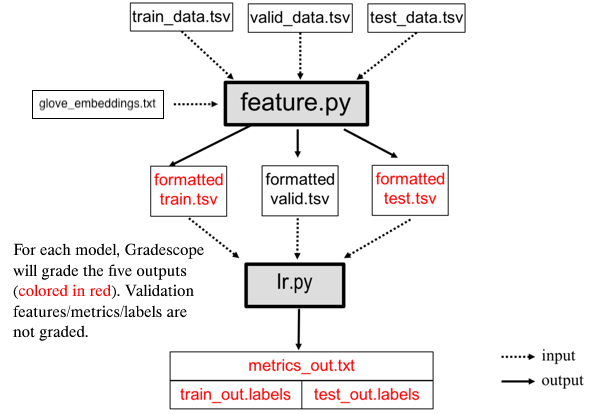
\includegraphics[width = 0.7\textwidth]{fig/Pipeline_v5.png}
        \caption{Programming pipeline for sentiment analyzer based on binary logistic regression}
        \label{pipeline}
\end{figure}

\subsection{Command Line Arguments}\label{commandline}
The autograder runs and evaluates the output from the files generated, using the following command (note \lstinline{feature} will be run before \lstinline{lr}):

\begin{tabbing}
\=\texttt{\$ \textbf{python} feature.\textbf{py} [args1\dots]}\\
\>\texttt{\$ \textbf{python} lr.\textbf{py} [args2\dots]}
\end{tabbing}

Where above \texttt{[args1\dots]} is a placeholder for seven command-line arguments: \texttt{<train\_input>}\newline \texttt{<validation\_input> <test\_input>  <feature\_dictionary\_input> \newline <formatted\_train\_out> <formatted\_validation\_out>  <formatted\_test\_out> }. These arguments are described in detail below:
\begin{enumerate}
    \item \texttt{<train\_input>}: path to the training input \texttt{.tsv} file (see Section~\ref{task})
    \item \texttt{<validation\_input>}: path to the validation input \texttt{.tsv} file (see Section~\ref{task})
    \item \texttt{<test\_input>}: path to the test input \texttt{.tsv} file (see Section~\ref{task})
    \item \texttt{<feature\_dictionary\_input>}: path to the \emph{GloVe} feature dictionary \texttt{.txt} file (see Section~\ref{featuremodels})
    \item \texttt{<formatted\_train\_out>}: path to output \texttt{.tsv} file to which the feature extractions on the \emph{training} data should be written (see Section~\ref{featurepy})
    \item \texttt{<formatted\_validation\_out>}: path to output \texttt{.tsv} file to which the feature extractions on the \emph{validation} data should be written (see Section~\ref{featurepy})
    \item \texttt{<formatted\_test\_out>}: path to output \texttt{.tsv} file to which the feature extractions on the \emph{test} data should be written (see Section~\ref{featurepy})
\end{enumerate}


Likewise, \texttt{[args2\dots]} is a placeholder for eight command-line arguments: \texttt{<formatted\_train\_input>} \texttt{<formatted\_validation\_input> <formatted\_test\_input> <train\_out> <test\_out> <metrics\_out> <num\_epoch> <learning\_rate>}. These arguments are described in detail below:
\begin{enumerate}
    \item \texttt{<formatted\_train\_input>}: path to the formatted training input \texttt{.tsv} file (see Section~\ref{featurepy})
    \item \texttt{<formatted\_validation\_input>}: path to the formatted validation input \texttt{.tsv} file (see Section~\ref{featurepy})
    \item \texttt{<formatted\_test\_input>}: path to the formatted test input \texttt{.tsv} file (see Section~\ref{featurepy})
    \item \texttt{<train\_out>}: path to output \texttt{.txt} file to which the prediction on the \emph{training} data should be written (see Section~\ref{lrpy})
    \item \texttt{<test\_out>}: path to output \texttt{.txt} file to which the prediction on the \emph{test} data should be written (see Section~\ref{lrpy})
    \item \texttt{<metrics\_out>}: path of the output \texttt{.txt} file to which metrics such as train and test error should be written (see Section~\ref{lrpy})
    \item \texttt{<num\_epoch>}: integer specifying the number of times SGD loops through all of the training data (e.g., if \texttt{<num\_epoch>} equals 5, then each training example will be used in SGD 5 times). 
    \item \texttt{<learning\_rate>}: float specifying the learning rate; in the reference output, we set the learning rate to be $0.1$ for all datasets
\end{enumerate}

As an example, the following two command lines would run your programs on the large dataset in the handout for 500 epochs. You are given the output of this command and the equivalent command on the small dataset in the handout directories \verb|largeoutput| and \verb|smalloutput|.

\begin{lstlisting}[language=Shell]
$ python feature.py \ 
largedata/train_large.tsv \
largedata/val_large.tsv \
largedata/test_large.tsv \
glove_embeddings.txt \
largeoutput/formatted_train_large.tsv \
largeoutput/formatted_val_large.tsv \
largeoutput/formatted_test_large.tsv

$ python lr.py \
largeoutput/formatted_train_large.tsv \
largeoutput/formatted_val_large.tsv \
largeoutput/formatted_test_large.tsv \
largeoutput/formatted_train_labels.txt \
largeoutput/formatted_test_labels.txt \
largeoutput/formatted_metrics.txt \
500 \
0.1
\end{lstlisting}

\begin{notebox}
{\bf Important Note:} You will not be writing out the predictions on validation data, only on train and test data. The validation data is \emph{only} used to give you an estimate of held-out negative log-likelihood at the end of each epoch during training. You are asked to graph the negative log-likelihood vs. epoch of the validation and training data in Programming Empirical Questions section. \footnote{For this assignment, we will always specify the number of epochs. However, a more mature implementation would monitor the performance on validation data at the end of each epoch and stop SGD when this validation log-likelihood appears to have converged. You should \textbf{\emph{not}} implement such a convergence check for this assignment.} 
\end{notebox}

\subsection{Starter Code}\label{startercode}

To help you start this assignment, we have provided starter code in the handout.



\subsection{Gradescope Submission }
You should submit your \texttt{feature.py} and \texttt{lr.py} to Gradescope.
\textit{Note}: please do not zip them or use other file names. This will cause problems for the autograder to correctly detect and run your code. Gradescope will also provide \textbf{hints for common bugs}; Ctrl-F for HINT if you did not receive a full score.
\newpage

\end{document}